% A float that the thesis shows in the main text and the manuscript in the appendix (\movedfloat).
\begin{figure}[htbp]\centering
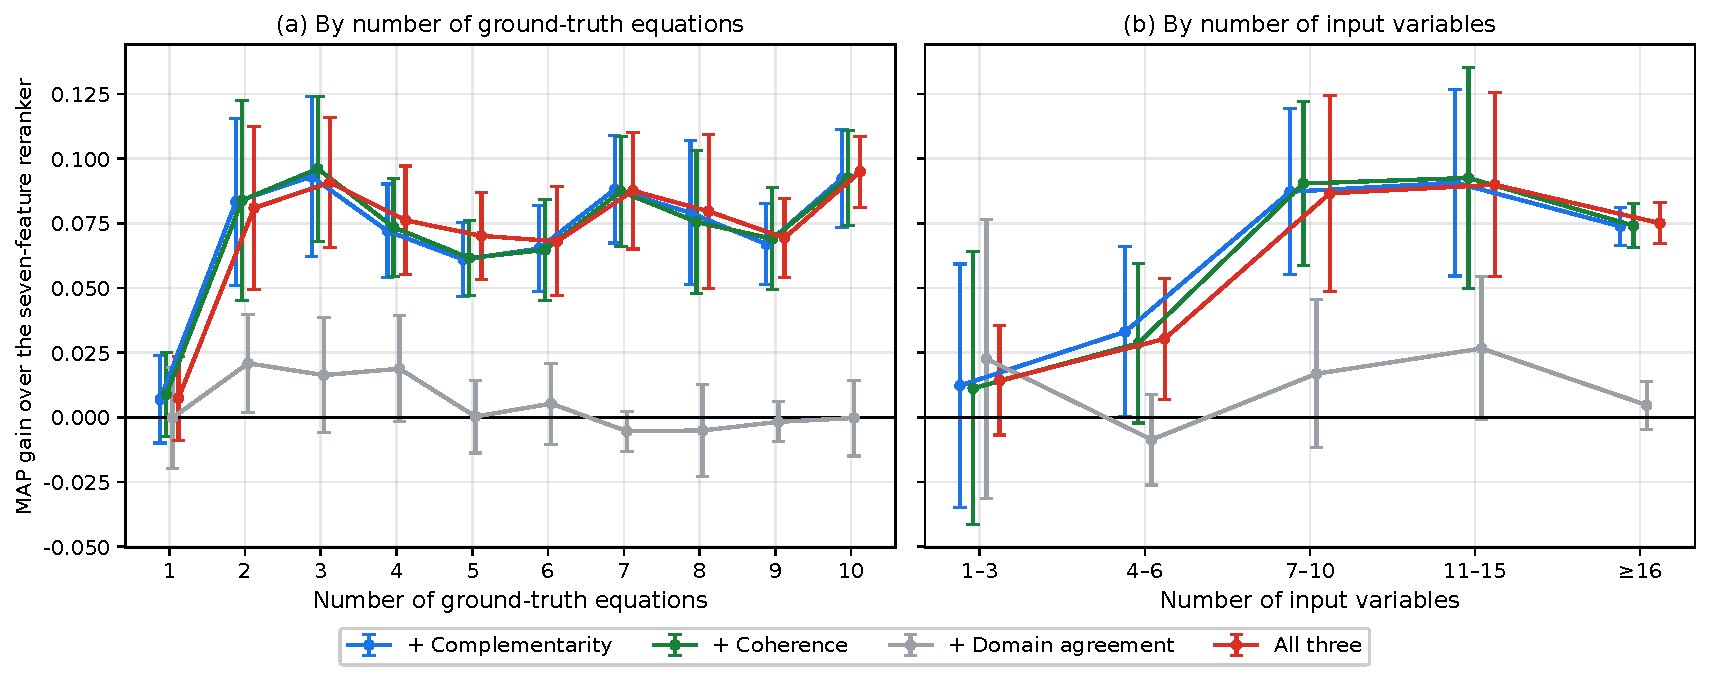
\includegraphics[width=\linewidth]{figures/fig_mechanism.pdf}
\caption{MAP gain over the reranker with the seven query--equation features when the set-aware
features are added one at a time or all three together (Setting~A), (a) by the number of
ground-truth equations and (b) by the number of input variables, in bins that differ from those
of Fig.~\ref{fig:characteristic}. Points show the mean over the 10 splits of the paired difference,
and error bars its SD across the splits.}
\label{fig:mechanism}
\end{figure}
